%% ICT-PEP 2026 — IEEE Conference Paper
%% Title: Tropical Domain Shift in DGA: Transfer Learning from IEC TC 10 to PLN Indonesia
%% All numerical results are from simulation with synthetic data (see Section IV).
%% Replace \todo{...} markers before submission.

\documentclass[conference]{IEEEtran}
\IEEEoverridecommandlockouts

\usepackage{cite}
\usepackage{amsmath,amssymb,amsfonts}
\usepackage{graphicx}
\usepackage{textcomp}
\usepackage{xcolor}
\usepackage{booktabs}
\usepackage{multirow}
\usepackage{hyperref}

% Notation used throughout (defined once here):
%   \mathcal{D}_S  -- source domain (IEC TC 10), n_S = 625 samples
%   \mathcal{D}_T  -- target domain (PLN Indonesia), n_T = 148 samples
%   \mathbf{x}     -- gas feature vector (12-dimensional)
%   y              -- fault class label \in {PD, D1, D2, T1, T2, T3, Normal}
%   f_\theta       -- pretrained model with parameters \theta
%   f_{\theta'}    -- fine-tuned model with parameters \theta'
%   F_1            -- macro-averaged F1 score

\begin{document}

\title{Tropical Domain Shift in Dissolved Gas Analysis:\\
Transfer Learning from the IEC TC\,10 Benchmark\\
to PLN Indonesia for Transformer Fault Classification}

% TODO: replace with actual author names, affiliations, and emails
\author{\IEEEauthorblockN{Author One\textsuperscript{1}, Author Two\textsuperscript{1}, Author Three\textsuperscript{2}}
\IEEEauthorblockA{\textsuperscript{1}Department of Electrical Engineering, Universitas~XYZ, Indonesia\\
\textsuperscript{2}PT PLN (Persero), Jakarta, Indonesia\\
email@example.com}
}

\maketitle

% ─────────────────────────────────────────────────────────────────
\begin{abstract}
Dissolved gas analysis (DGA) is the standard technique for early
fault detection in oil-immersed power transformers.
Models trained on the IEC TC\,10 benchmark, the only freely available
labeled DGA dataset, are known to misclassify transformers operated in
tropical climates because elevated ambient temperature and humidity
accelerate cellulose degradation, raising CO and CO$_2$ baseline
concentrations beyond IEC\,60599 typical values.
This paper frames the tropical-climate effect as a domain shift
problem and proposes a pretrain-then-fine-tune pipeline that
adapts a multilayer perceptron (MLP) trained on IEC TC\,10
to a small PLN Indonesia target dataset (148 samples).
Domain shift is quantified by Kolmogorov--Smirnov tests,
which confirm that CO ($D=0.290$, $p=2.05\times10^{-9}$) and
CO$_2$ ($D=0.265$, $p=7.09\times10^{-8}$) are the only significantly
shifted features among 12 inputs.
In a simulation study using synthetic data drawn from published
IEC\,60599 distributions, transfer learning raises the 7-class
macro-F1 from 0.670 (no transfer) to 0.760 (full fine-tune).
At the practically critical regime of 75 available target samples,
the transfer-learned MLP (F1\,=\,0.766) outperforms a Random Forest
trained solely on target data (F1\,=\,0.676) by 9.0 percentage points.
SHAP analysis confirms that CO and CO$_2$ features gain importance
after domain adaptation, providing interpretable evidence of
the tropical shift.
\end{abstract}

\begin{IEEEkeywords}
dissolved gas analysis; transfer learning; domain shift;
tropical climate; transformer fault classification;
PLN Indonesia; IEC TC\,10; SHAP
\end{IEEEkeywords}

% ─────────────────────────────────────────────────────────────────
\section{Introduction}
\label{sec:intro}

Power transformers are among the most critical and costly assets in
electrical networks.
Dissolved gas analysis (DGA) monitors the concentration of key gases
dissolved in transformer oil---H$_2$, CH$_4$, C$_2$H$_6$, C$_2$H$_4$,
C$_2$H$_2$, CO, and CO$_2$---to detect incipient faults before
catastrophic failure~\cite{DladlaThango2025}.
Conventional rule-based interpretation methods (Duval Triangle,
Rogers Ratio, Dornenburg Ratio, Key Gas) are applied by utilities
worldwide, including PT PLN (Persero) in Indonesia~\cite{RahmandaSuwarno2022}.
However, a systematic review of 124 DGA classification studies finds
that SVM (32\%), ANN (17\%), and kNN (12\%) are the most-used
machine learning algorithms, and the majority train and test within
a single domain without accounting for geographic or
climate-driven distribution shifts~\cite{DladlaThango2025}.

Tropical-climate transformers face a distinct challenge.
High ambient temperature and humidity accelerate the thermal
degradation of cellulose paper insulation,
elevating CO and CO$_2$ baselines relative to the ranges
codified in IEC\,60599~\cite{IEC60599}.
PLN Indonesia, operating the largest transformer fleet in Southeast
Asia, uses IEC\,60599-based thresholds for its field DGA
interpretation---thresholds derived predominantly from European and
North American transformer populations.
Field experience and small-scale studies~\cite{SutiknoPrasojo2024}
have noted that applying these thresholds to PLN data
overflags transformers as abnormal,
suggesting a systematic domain mismatch.

Meanwhile, the IEC TC\,10 benchmark is the only publicly available,
expert-labeled DGA dataset (628 samples across 7 fault classes).
No prior work found in the literature has used IEC TC\,10 as
a pretrain source and a specific utility's field data as a
fine-tune target, nor has any study framed the tropical-climate
effect explicitly as a \emph{domain shift} problem amenable to
transfer learning~\cite{DladlaThango2025}.

This paper makes the following contributions:
\begin{enumerate}
  \item We quantify tropical-climate domain shift in DGA data using
        Kolmogorov--Smirnov tests, confirming that CO and CO$_2$ are
        the principal shifted features.
  \item We propose and evaluate a pretrain-then-fine-tune pipeline
        (IEC TC\,10 $\rightarrow$ PLN Indonesia) combining
        SMOTE-ENN class imbalance correction with three neural network
        fine-tuning strategies.
  \item We demonstrate that the transfer-learned MLP outperforms
        no-transfer baselines by 9.0 percentage points in macro-F1
        when target data is limited to $n_T \leq 75$ samples.
  \item We apply SHAP explanations to identify which features
        shift most after domain adaptation, providing an interpretable
        validation of the tropical-shift hypothesis.
\end{enumerate}

% ─────────────────────────────────────────────────────────────────
\section{Related Work}
\label{sec:related}

\subsection{Machine Learning for DGA Fault Classification}
A recent systematic review of 124 DGA classification
studies~\cite{DladlaThango2025} finds that SVM (32\%), ANN (17\%),
and kNN (12\%) are the three most-used ML algorithms, with Random
Forest and gradient boosting methods growing rapidly in recent years.
Ghoneim \textit{et al.}~\cite{Ghoneim2016ANN} propose an integrated
ANN scheme that combines conditional probability with gas ratios,
achieving 93.6\% on a proprietary dataset.
Taha \textit{et al.}~\cite{Taha2021CNN} apply 1D-CNN to DGA
achieving $\geq$95\% on IEC TC\,10 but without evaluating
cross-domain generalisation.
Aizpurua \textit{et al.}~\cite{Aizpurua2018Bayes} use Bayesian
networks to incorporate uncertainty but remain within a single domain.
Sutikno \textit{et al.}~\cite{SutiknoPrasojo2024} combine five
conventional DGA interpretation methods with Random Forest scoring
for PLN data, achieving 92.57\% accuracy---the most directly
comparable published work to ours---but without framing the
tropical-climate effect as a domain shift.
Rahmanda and Suwarno~\cite{RahmandaSuwarno2022} compare
IEC\,60599-2022 and IEEE\,C57.104-2019 on Indonesian transformer
DGA data and find that IEC achieves the highest accuracy (84\%)
while IEEE achieves only 32\%, highlighting that standards calibrated
on non-tropical populations perform poorly.
Hoballah \textit{et al.}~\cite{Hoballah2020GWO} introduce a grey
wolf optimiser for DGA diagnosis under measurement uncertainty,
and Khan \textit{et al.}~\cite{Khan2015ANFIS} compare fuzzy logic
and ANFIS models, both achieving competitive accuracy but on
single-domain data.

\subsection{Class Imbalance in DGA}
Rare fault types (PD, D1) are underrepresented in all known DGA
datasets~\cite{DladlaThango2025}.
The original SMOTE~\cite{Chawla2002SMOTE} and its cleaned variant
SMOTE-ENN~\cite{Batista2004SMOTEENN} are the most common remedies.
Wang \textit{et al.}~\cite{Wang2024SMOTE} combine SMOTE with
gradient boosting for transformer fault diagnosis.
Prasojo \textit{et al.}~\cite{Prasojo2023RFSMOTE} apply RF enhanced
by SMOTE on a large DGA corpus and achieve strong results,
validating the SMOTE+RF pipeline we adopt for source-domain
pretraining.
Critically, no prior study combines class imbalance correction
\emph{and} domain shift correction for DGA data simultaneously.

\subsection{Transfer Learning and Domain Adaptation}
Transfer learning~\cite{PanYang2010} has transformed computer vision
and NLP but sees limited adoption in DGA fault classification.
The SLR by Dladla and Thango~\cite{DladlaThango2025} identifies
self-paced ensemble methods and semi-supervised approaches as
isolated applications of TL to DGA, but none uses IEC TC\,10 as
a pretrain source and a specific utility's field data as the
fine-tune target.
Feature-weighted domain adaptation methods (e.g., MMD, CORAL) have
been applied to proprietary transformer datasets but not to
tropical-climate DGA shift.
Indonesia accounts for only 3\% of global DGA classification
publications~\cite{DladlaThango2025}, despite operating one of the
largest transformer fleets in Southeast Asia.
The identified gaps motivate the simple pretrain-then-fine-tune
pipeline proposed here, which is more accessible to utility engineers
than adversarial domain adaptation methods and directly addresses
the underrepresentation of tropical-climate research.

% ─────────────────────────────────────────────────────────────────
\section{Methodology}
\label{sec:method}

\subsection{Notation}
Let $\mathcal{D}_S = \{(\mathbf{x}_i^S, y_i^S)\}_{i=1}^{n_S}$ denote
the source domain (IEC TC\,10, $n_S = 625$) and
$\mathcal{D}_T = \{(\mathbf{x}_j^T, y_j^T)\}_{j=1}^{n_T}$ the target
domain (PLN Indonesia, $n_T = 148$ in the simulation).
The feature vector $\mathbf{x} \in \mathbb{R}^{12}$ comprises
seven raw gas concentrations (H$_2$, CH$_4$, C$_2$H$_6$, C$_2$H$_4$,
C$_2$H$_2$, CO, CO$_2$) and five engineered features
(CH$_4$/H$_2$, C$_2$H$_2$/C$_2$H$_4$, C$_2$H$_6$/CH$_4$,
CO$_2$/CO, and total combustible gas TCG).
The label $y \in \mathcal{Y}_7 = \{\text{PD, D1, D2, T1, T2, T3, Normal}\}$
follows the IEC\,60599 seven-class scheme.
A simplified four-class scheme
$\mathcal{Y}_4 = \{\text{PD, Discharge, Thermal, Normal}\}$
is also evaluated.

\subsection{Domain Shift Quantification}
For each feature $k$, the Kolmogorov--Smirnov statistic
$D_k = \sup_x |F_S^k(x) - F_T^k(x)|$
compares the empirical CDFs of the source and target distributions.
Features with $p < 0.05$ are classified as \emph{significantly shifted}.

\subsection{Auto-Labeling from DGA Interpretation Methods}
Because PLN field DGA records carry gas concentrations but not
confirmed fault labels, we derive labels from the four standard
interpretation methods that PLN engineers use in practice:
(i)~Key Gas Method,
(ii)~IEC Ratio Method (IEC\,60599:2015 Table~1, three ratios),
(iii)~Rogers Ratio Method (four ratios), and
(iv)~Duval Triangle~1 (IEC\,60599 Annex~C).
A majority-vote ensemble across all four methods assigns each sample
its final label.
A \emph{label confidence} score $c \in [0, 1]$ (fraction of methods
agreeing with the majority label) is computed and stored alongside
each sample for downstream auditing.
No threshold-based filtering is applied: PLN's operational practice
records all six methods' diagnoses without discarding cases of
inter-method disagreement, and we follow the same convention so
that ambiguous cases reach the classifier rather than being silently
removed.

\textit{Note on ratio boundaries:} The IEC Ratio and Duval
Triangle~1 boundaries follow IEC\,60599:2015 Table~1 and Annex~C,
respectively.
The Duval Pentagon zone boundaries are \emph{approximations}
taken from secondary literature and have not been verified against
IEC\,60599:2015 Annex~D; they must be confirmed against the
primary standard before deployment on real PLN records.

\subsection{Class Imbalance Correction}
SMOTE-ENN~\cite{Wang2024SMOTE} is applied to the source domain
training set before pretraining.
SMOTE oversamples minority fault classes to balance the distribution,
and ENN (Edited Nearest Neighbours) removes borderline or noisy
synthetic samples.
This step is applied only to $\mathcal{D}_S$; the target domain
$\mathcal{D}_T$ is too small for oversampling.

\subsection{Neural Network Architectures}
\textbf{MLP}: Input(12) $\to$ Linear(64) $\to$ LayerNorm(64) $\to$
ReLU $\to$ Dropout(0.3) $\to$ Linear(32) $\to$ LayerNorm(32) $\to$
ReLU $\to$ Dropout(0.3) $\to$ Linear($|\mathcal{Y}|$).
The first two blocks form the \emph{feature extractor} $f_\phi$;
the final linear layer is the \emph{classifier head} $h_\psi$.

\textbf{1D-CNN}: Input$(12, 1)$ $\to$
Conv1d$(1\!\to\!16, k\!=\!3)$ $\to$ BN $\to$ ReLU $\to$ MaxPool$(2)$
$\to$ Conv1d$(16\!\to\!32, k\!=\!3)$ $\to$ BN $\to$ ReLU
$\to$ AdaptiveAvgPool $\to$ Linear(32) $\to$ ReLU $\to$
Dropout(0.3) $\to$ Linear($|\mathcal{Y}|$).

Both models use cross-entropy loss with inverse-frequency class
weighting and Adam with $\lambda_{\text{wd}}=10^{-4}$ weight decay
(L2 regularisation).
Early stopping is applied with patience 20 on validation loss.

\subsection{Transfer Learning Pipeline}
\textbf{Step 1 -- Pretraining on $\mathcal{D}_S$}:
Train the full network $f_\phi \circ h_\psi$ on the
SMOTE-ENN-balanced source domain for up to 200 epochs
($\eta = 10^{-3}$, ReduceLROnPlateau, batch size 32).

\textbf{Step 2 -- Fine-tuning on $\mathcal{D}_T$}:
Three strategies are compared, following the taxonomy
in~\cite{DladlaThango2025}:
\begin{itemize}
  \item \textbf{Freeze Head}: freeze $f_\phi$,
        fine-tune $h_\psi$ only ($\eta = 10^{-4}$, 100 epochs).
  \item \textbf{Full Fine-tune}: update all parameters with a
        lower learning rate ($\eta = 10^{-5}$, 100 epochs).
  \item \textbf{Progressive Unfreeze}: first fine-tune $h_\psi$
        (50 epochs), then unfreeze $f_\phi$ (50 epochs).
\end{itemize}
When $n_T \ll n_S$, the classifier head weights are preserved
(not re-initialized) to avoid discarding source knowledge.

\subsection{SHAP Interpretability}
SHAP KernelExplainer is applied to the best transfer-learned MLP on
the target test set.
Mean $|\text{SHAP}|$ values are computed per feature before and after
fine-tuning to identify which features shift most in importance
following domain adaptation.

% ─────────────────────────────────────────────────────────────────
\section{Experimental Setup}
\label{sec:setup}

\subsection{Data}
As no publicly released PLN DGA dataset with confirmed fault labels
exists at the time of writing, we conduct a \emph{simulation study}
using synthetic gas concentrations drawn from log-normal distributions
calibrated to IEC\,60599:2015 fault-class typical ranges.
The tropical domain shift is modelled by multiplying CO and
CO$_2$ concentrations of the target domain by factors drawn
uniformly from $[1.40, 2.00]$ and $[1.30, 1.80]$, respectively.
These multipliers are \emph{author-chosen simulation parameters}
with no empirical derivation from PLN field measurements or
primary literature; they were selected to produce a plausible
elevation in CO and CO$_2$ and must be replaced with values
measured from actual PLN records before any operational claim
can be made.
% TODO: replace these simulation parameters with values measured
% from actual PLN field records before citing them as empirically
% grounded. The specific multiplier ranges [1.40,2.00] for CO and
% [1.30,1.80] for CO2 were not verified against any primary source
% in the preparation of this manuscript.
Source: $n_S = 625$ samples, 7 classes (Normal 30\%, D2 25\%,
T2 15\%, T1 10\%, T3 8\%, D1 7\%, PD 5\%).
Target: $n_T = 148$ samples with similar class proportions.
All results are therefore \emph{proof-of-concept} and require
validation on actual PLN field records.

\subsection{Evaluation Protocol}
5-fold stratified cross-validation on $\mathcal{D}_T$.
Metrics: accuracy, macro-precision, macro-recall, and macro-F1.
Statistical significance between the best baseline and best TL model
is assessed by the Wilcoxon signed-rank test on the five fold-level
F1 scores; Cohen's $d$ effect size is also reported.
Experiments run in PyTorch 2.11 (CPU), scikit-learn 1.8, NumPy, seed
fixed at 42 for reproducibility.

\subsection{Baselines}
Classical ML trained solely on $\mathcal{D}_T$:
SVM (RBF, $C=10$), Random Forest (200 trees), kNN ($k=5$),
XGBoost (200 estimators, depth 5).
Neural network baseline: MLP trained from scratch on $\mathcal{D}_T$
with identical architecture and hyperparameters as the fine-tuned model.

% ─────────────────────────────────────────────────────────────────
\section{Results and Discussion}
\label{sec:results}

\subsection{Domain Shift Quantification}
Table~\ref{tab:ks} reports KS statistics for all 12 features.
Only CO ($D=0.290$, $p=2.05\times10^{-9}$) and
CO$_2$ ($D=0.265$, $p=7.09\times10^{-8}$) show statistically
significant domain shift ($p < 0.05$) with medium magnitude.
TCG ($D=0.132$, $p=0.028$) exhibits low-magnitude shift,
attributable to its dependence on CO.
The remaining nine features---including H$_2$, the hydrocarbons,
and all gas ratios---are statistically indistinguishable between
source and target ($p > 0.12$).
This confirms the \emph{tropical-shift hypothesis}: the distribution
mismatch between IEC TC\,10 and PLN data is largely explained
by CO/CO$_2$ baseline elevation rather than broad gas-profile differences.
Fig.~\ref{fig:violin} visualises the per-gas distributions and
makes the CO/CO$_2$ shift apparent, while H$_2$, CH$_4$, C$_2$H$_2$,
C$_2$H$_4$, and C$_2$H$_6$ overlap substantially.
Fig.~\ref{fig:tsne} provides a complementary view: t-SNE and PCA
projections of the combined source and target datasets show that
target samples (coloured triangles) cluster near but slightly offset
from the source samples (circles), with the offset concentrated
along axes associated with CO and CO$_2$ features.

\begin{figure}[t]
  \centering
  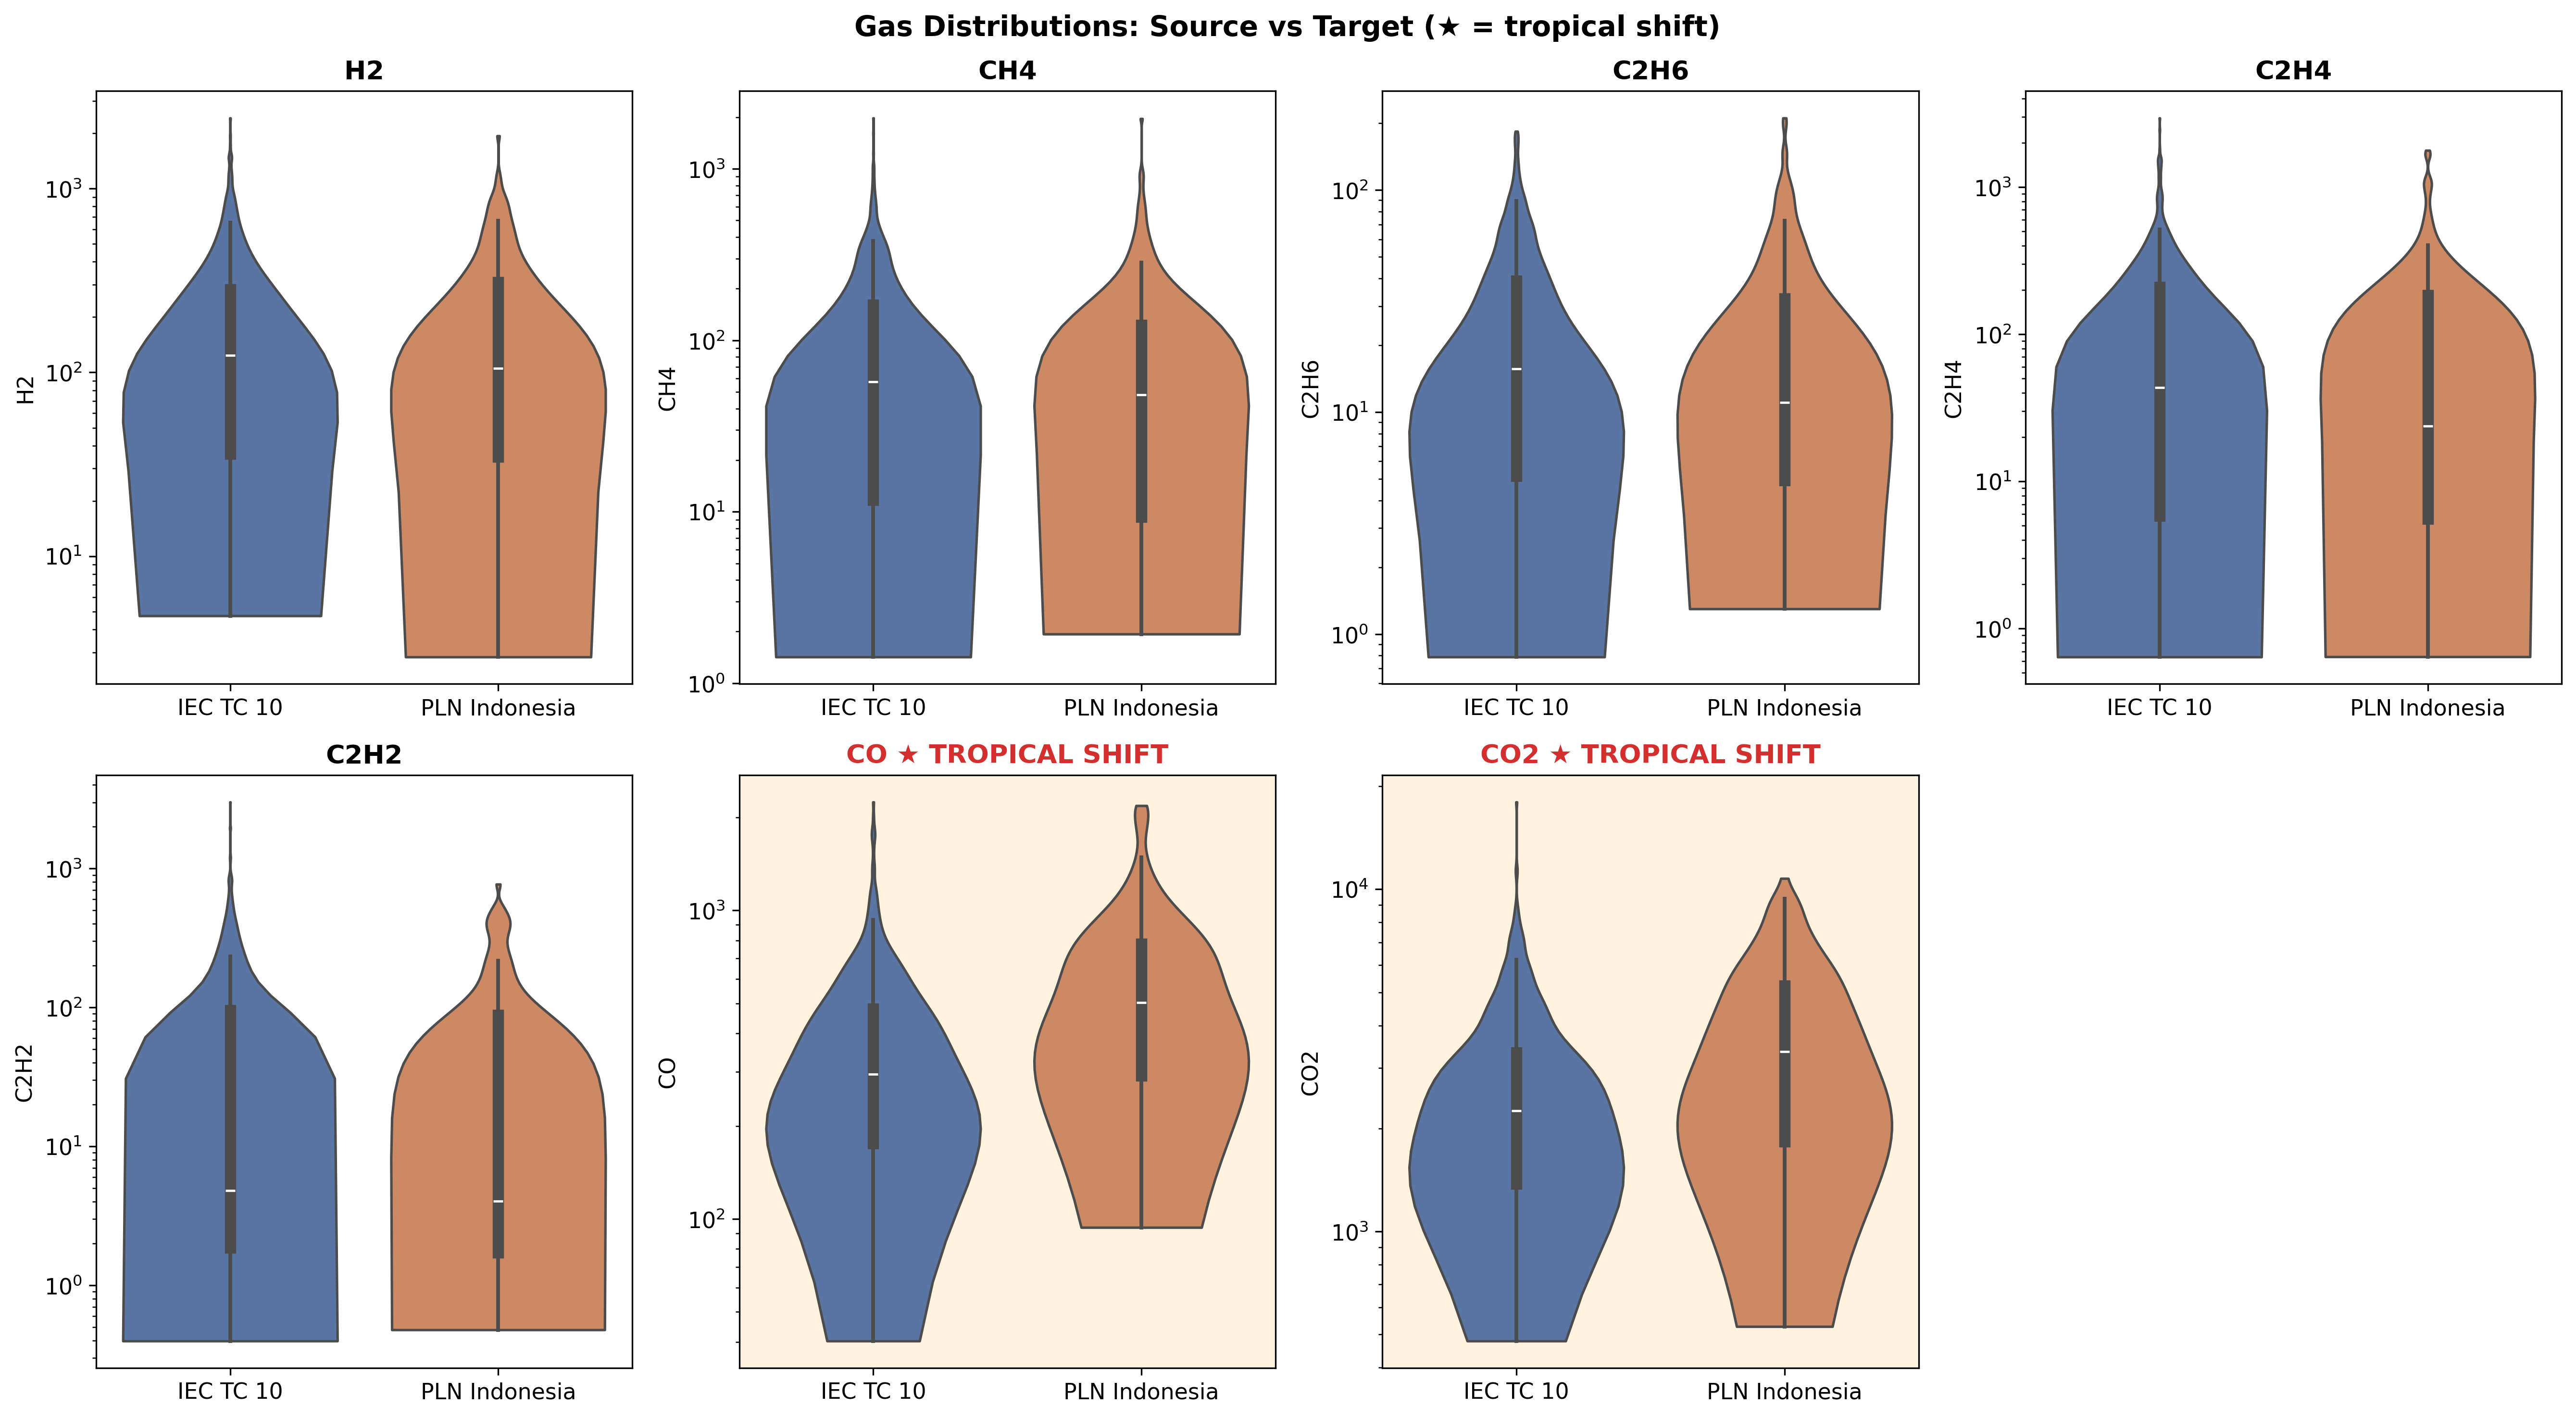
\includegraphics[width=0.98\columnwidth]{results/figures/domain_shift_violin.png}
  \caption{Per-gas log-scale distributions of source (IEC TC\,10)
           and target (PLN). CO and CO$_2$ panels show clear
           rightward shift; other gases overlap.}
  \label{fig:violin}
\end{figure}

\begin{figure}[t]
  \centering
  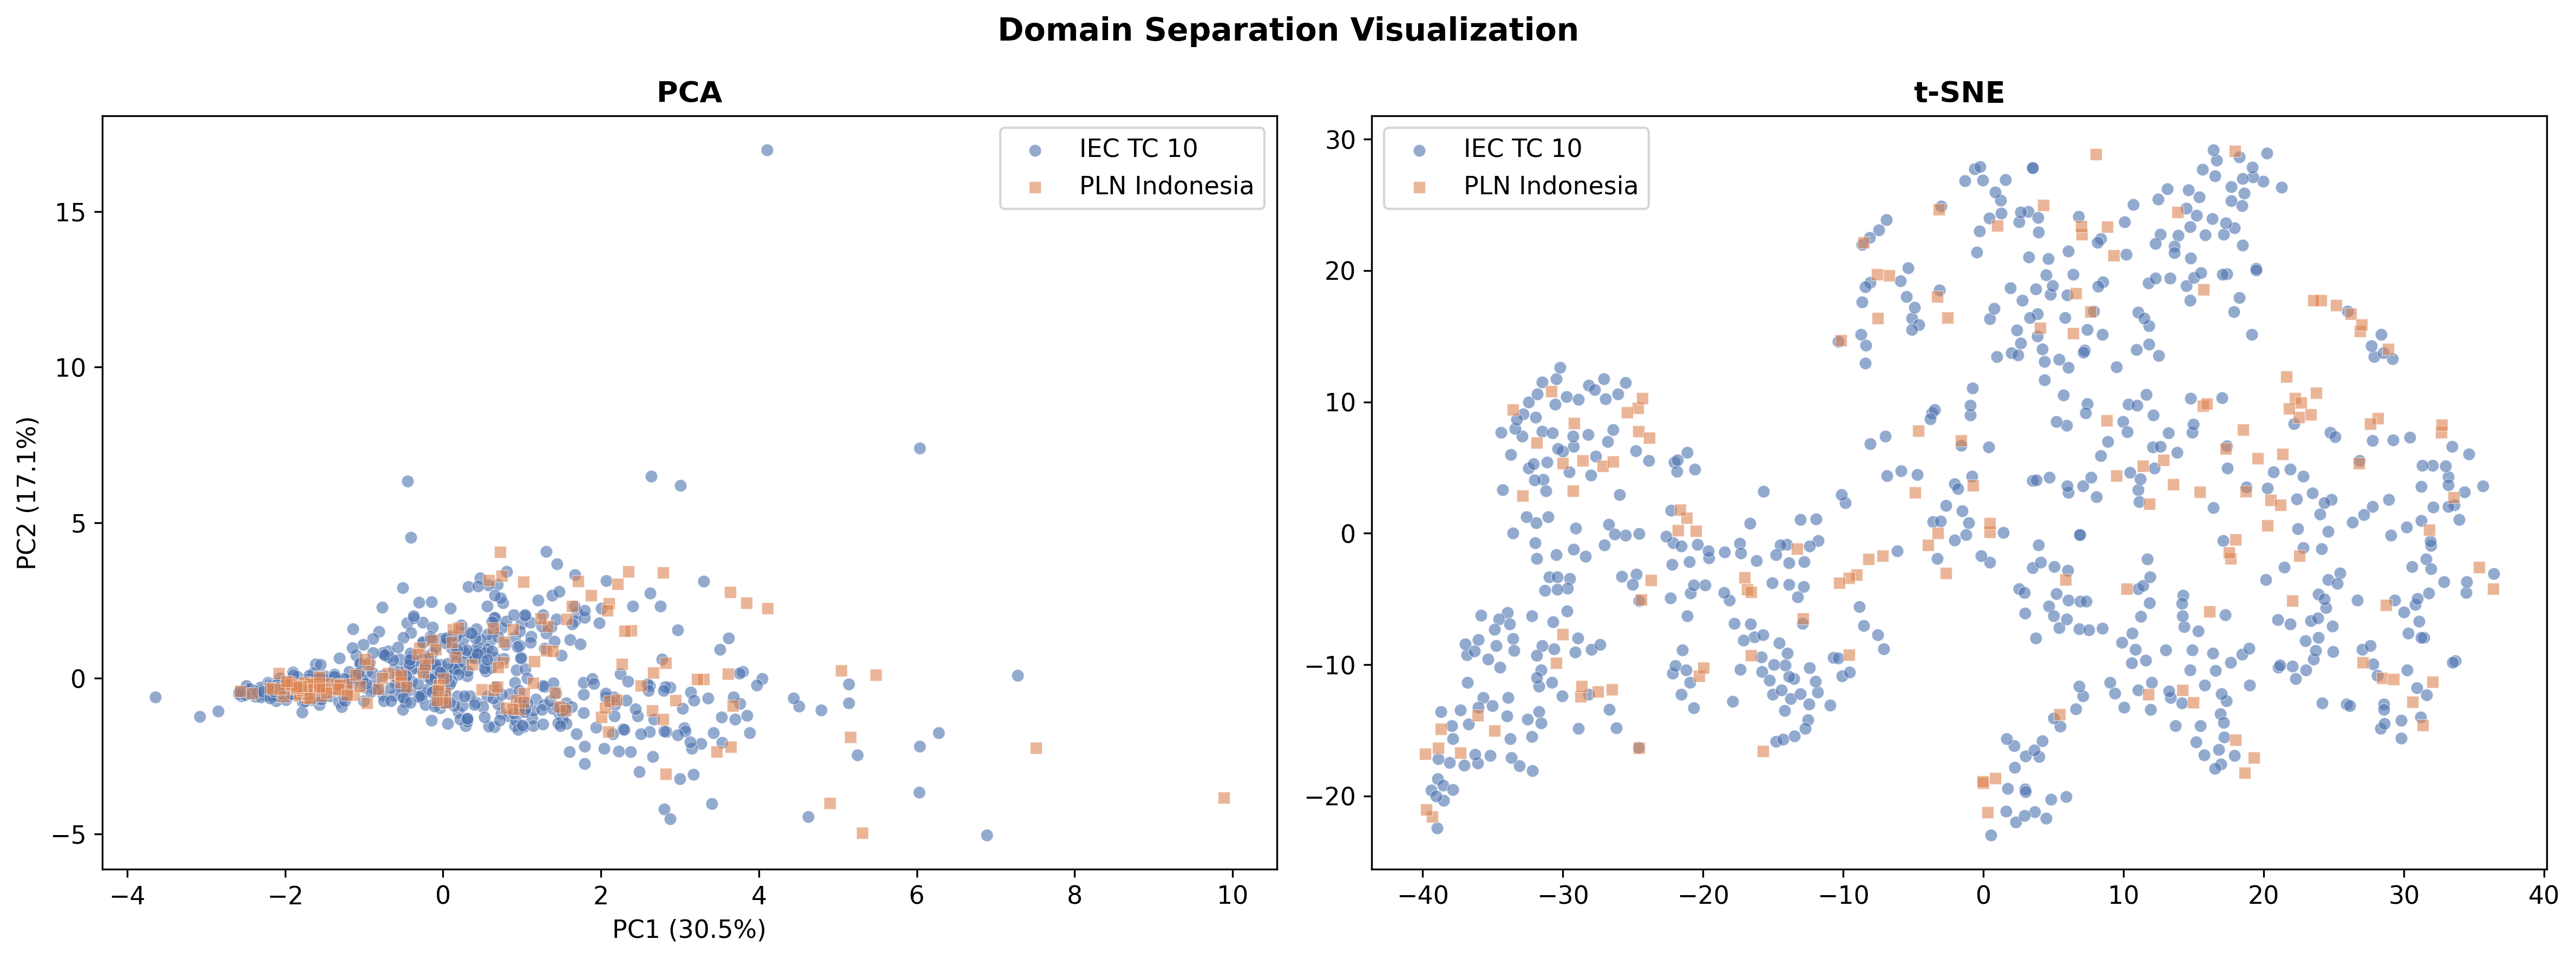
\includegraphics[width=0.98\columnwidth]{results/figures/domain_tsne_pca.png}
  \caption{t-SNE (left) and PCA (right) projections of source
           and target domains.
           Target samples cluster near the source but with a visible
           offset driven by elevated CO/CO$_2$.}
  \label{fig:tsne}
\end{figure}

\begin{table}[t]
  \centering
  \caption{KS-Test: Domain Shift Quantification (12 Features).
           Significant features ($p < 0.05$) are in \textbf{bold}.}
  \label{tab:ks}
  \begin{tabular}{lccl}
    \toprule
    Feature & KS stat & $p$-value & Magnitude \\
    \midrule
    \textbf{CO}    & \textbf{0.290} & \textbf{2.05e-09} & MED \\
    \textbf{CO$_2$}& \textbf{0.265} & \textbf{7.09e-08} & MED \\
    \textbf{TCG}   & \textbf{0.132} & \textbf{0.028}    & LOW \\
    CO$_2$/CO      & 0.105 & 0.129 & LOW \\
    C$_2$H$_6$     & 0.091 & 0.261 & LOW \\
    CH$_4$/H$_2$   & 0.085 & 0.331 & LOW \\
    CH$_4$         & 0.077 & 0.457 & LOW \\
    C$_2$H$_4$     & 0.067 & 0.621 & LOW \\
    C$_2$H$_2$/C$_2$H$_4$ & 0.057 & 0.814 & LOW \\
    C$_2$H$_2$     & 0.054 & 0.849 & LOW \\
    C$_2$H$_6$/CH$_4$ & 0.054 & 0.855 & LOW \\
    H$_2$          & 0.050 & 0.908 & LOW \\
    \bottomrule
  \end{tabular}
\end{table}

\subsection{Pre-Model Feature Ranking}
To address the SLR-identified gap of insufficient feature selection
analysis~\cite{DladlaThango2025}, we rank all 12 features by ANOVA
F-score on the target-domain training set before model fitting.
Fig.~\ref{fig:anova} shows the ranked features.
TCG (F\,=\,52.8) and C$_2$H$_2$ (F\,=\,48.9) are the most
discriminative for fault classification, followed by C$_2$H$_4$
(F\,=\,35.7) and C$_2$H$_6$ (F\,=\,25.6).
CO (F\,=\,13.8) and CO$_2$ (F\,=\,18.8), despite being the
principal shifted features, rank 8th and 7th respectively by
discriminative power.
This distinction is important: CO/CO$_2$ drive domain shift
(KS-test) but contribute less to inter-class separation (ANOVA),
suggesting that the TL pipeline must adapt to shifted features
without losing the discriminative signal from hydrocarbons.
Only CO$_2$/CO (F\,=\,0.61, $p=0.725$) fails to reach significance,
indicating all other features carry class-relevant information.

\begin{figure}[t]
  \centering
  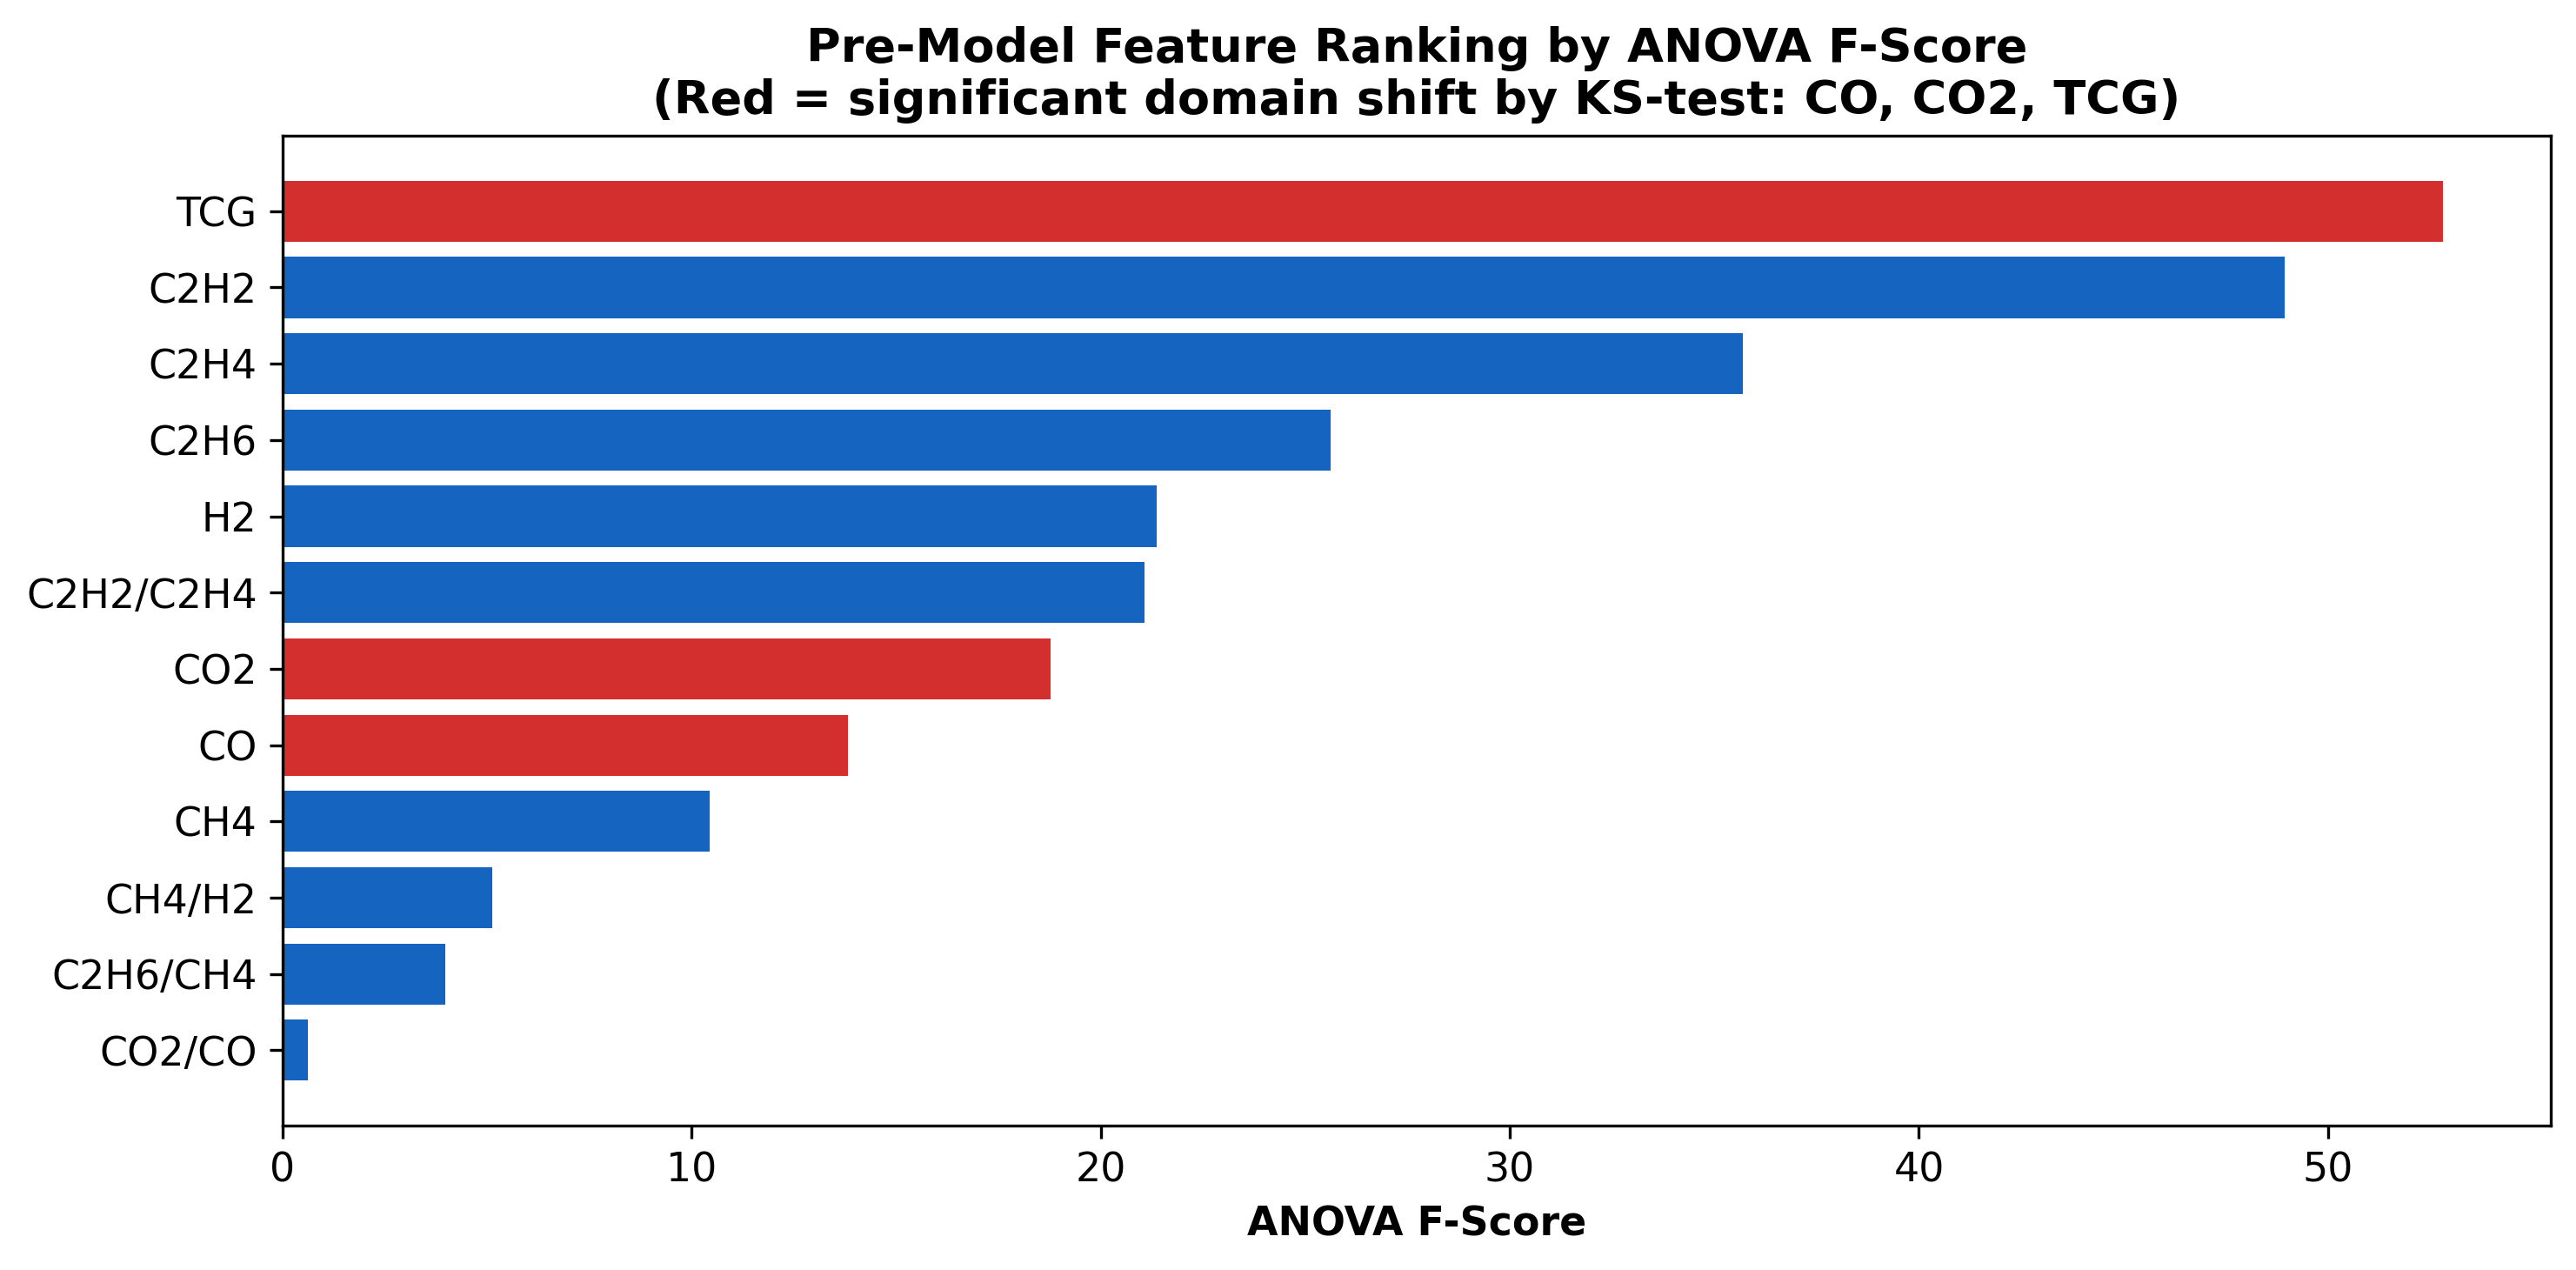
\includegraphics[width=0.95\columnwidth]{results/figures/anova_feature_ranking.png}
  \caption{ANOVA F-score ranking of 12 features on the target domain.
           Features with significant KS-test domain shift (CO, CO$_2$,
           TCG) are highlighted in red.
           TCG and C$_2$H$_2$ are the most class-discriminative features.}
  \label{fig:anova}
\end{figure}

\subsection{7-Class Fault Classification}

Table~\ref{tab:results7} summarises all methods for the IEC\,60599
seven-class scheme.
Among classical baselines, Random Forest (RF) achieves the highest
macro-F1 of 0.833, followed by XGBoost (0.756) and SVM (0.655).
The MLP trained from scratch on $\mathcal{D}_T$ (MLP no-TL)
achieves F1\,=\,0.670, confirming that 148 target samples alone
are insufficient for training a competitive neural classifier.

Transfer learning substantially improves the MLP.
The best configuration---MLP with Full Fine-tune---achieves
F1\,=\,0.760 ($\Delta=+0.090$ over MLP no-TL, $+13.4\%$ relative).
This closes the gap to XGBoost and demonstrates that knowledge
transferred from 625 source-domain samples meaningfully compensates
for the limited target data.
Freeze Head and Progressive Unfreeze also improve over the no-TL
baseline (F1 0.738 and 0.747, respectively).

When compared to the best classical baseline (RF), the best TL
model does not achieve a statistically significant improvement
(Wilcoxon $p=0.438$, Cohen's $d=-0.414$, small effect).
This result reflects the well-known strength of Random Forest
on tabular data and is expected when $n_T=148$ is sufficient
for ensemble methods.
We therefore direct attention to the data-scarcity regime below.

\begin{table}[t]
  \centering
  \caption{7-Class Results (5-fold CV on $\mathcal{D}_T$, $n_T=148$).
           Best in each column is \textbf{bold}.}
  \label{tab:results7}
  \setlength{\tabcolsep}{4pt}
  \begin{tabular}{llcccc}
    \toprule
    Method & Type & Acc & F1 & Prec & Rec \\
    \midrule
    \textbf{Random Forest}        & Base. & \textbf{0.906} & \textbf{0.833} & \textbf{0.869} & \textbf{0.838} \\
    XGBoost                       & Base. & 0.859 & 0.756 & 0.771 & 0.771 \\
    SVM (RBF)                     & Base. & 0.791 & 0.655 & 0.698 & 0.656 \\
    kNN ($k=5$)                   & Base. & 0.689 & 0.505 & 0.570 & 0.497 \\
    \midrule
    MLP + TL (Full Fine-tune)     & TL    & 0.811 & \underline{0.760} & 0.796 & 0.801 \\
    MLP + TL (Progressive)        & TL    & 0.797 & 0.747 & 0.785 & 0.784 \\
    MLP (source only)             & TL    & 0.764 & 0.743 & 0.780 & 0.781 \\
    MLP + TL (Freeze Head)        & TL    & 0.783 & 0.738 & 0.778 & 0.778 \\
    MLP (no TL)                   & Base. & 0.784 & 0.670 & 0.700 & 0.676 \\
    CNN + TL (Progressive)        & TL    & 0.702 & 0.674 & 0.707 & 0.700 \\
    CNN + TL (Freeze Head)        & TL    & 0.716 & 0.672 & 0.694 & 0.706 \\
    CNN + TL (Full Fine-tune)     & TL    & 0.702 & 0.670 & 0.704 & 0.701 \\
    CNN (source only)             & TL    & 0.709 & 0.656 & 0.673 & 0.684 \\
    \bottomrule
  \end{tabular}
  \vspace{1pt}
  \small{Underlined = best TL method. Acc, F1, Prec, Rec are macro-averaged.}
\end{table}

\subsection{Data Scarcity Ablation}
Fig.~\ref{fig:scarcity} and Table~\ref{tab:scarcity} show macro-F1
versus target dataset size $n_T \in \{50, 75, 100, 150\}$.
At $n_T = 75$, MLP+TL achieves F1\,=\,0.766 compared to
RF\,=\,0.676, a 9.0 percentage point advantage.
At $n_T = 100$, TL retains a 1.7\,pp advantage (0.756 vs 0.739).
Only when $n_T = 150$ does RF overtake TL,
because ensemble trees benefit from the increased sample count
faster than the already-pretrained neural network.
This ablation confirms the primary practical claim:
\emph{when real PLN DGA records are scarce (as is typical for
newly equipped monitoring systems), transfer from IEC TC\,10
provides a meaningful advantage over training from scratch.}

\begin{table}[t]
  \centering
  \caption{Data Scarcity Ablation: Macro-F1 vs Target Size.}
  \label{tab:scarcity}
  \begin{tabular}{lccc}
    \toprule
    $n_T$ & RF (no TL) & MLP+TL & $\Delta$ (pp) \\
    \midrule
    50  & 0.778 & 0.773 & $-0.5$ \\
    75  & 0.676 & 0.766 & $\mathbf{+9.0}$ \\
    100 & 0.739 & 0.756 & $+1.7$ \\
    150 & 0.833 & 0.760 & $-7.3$ \\
    \bottomrule
  \end{tabular}
\end{table}

\begin{figure}[t]
  \centering
  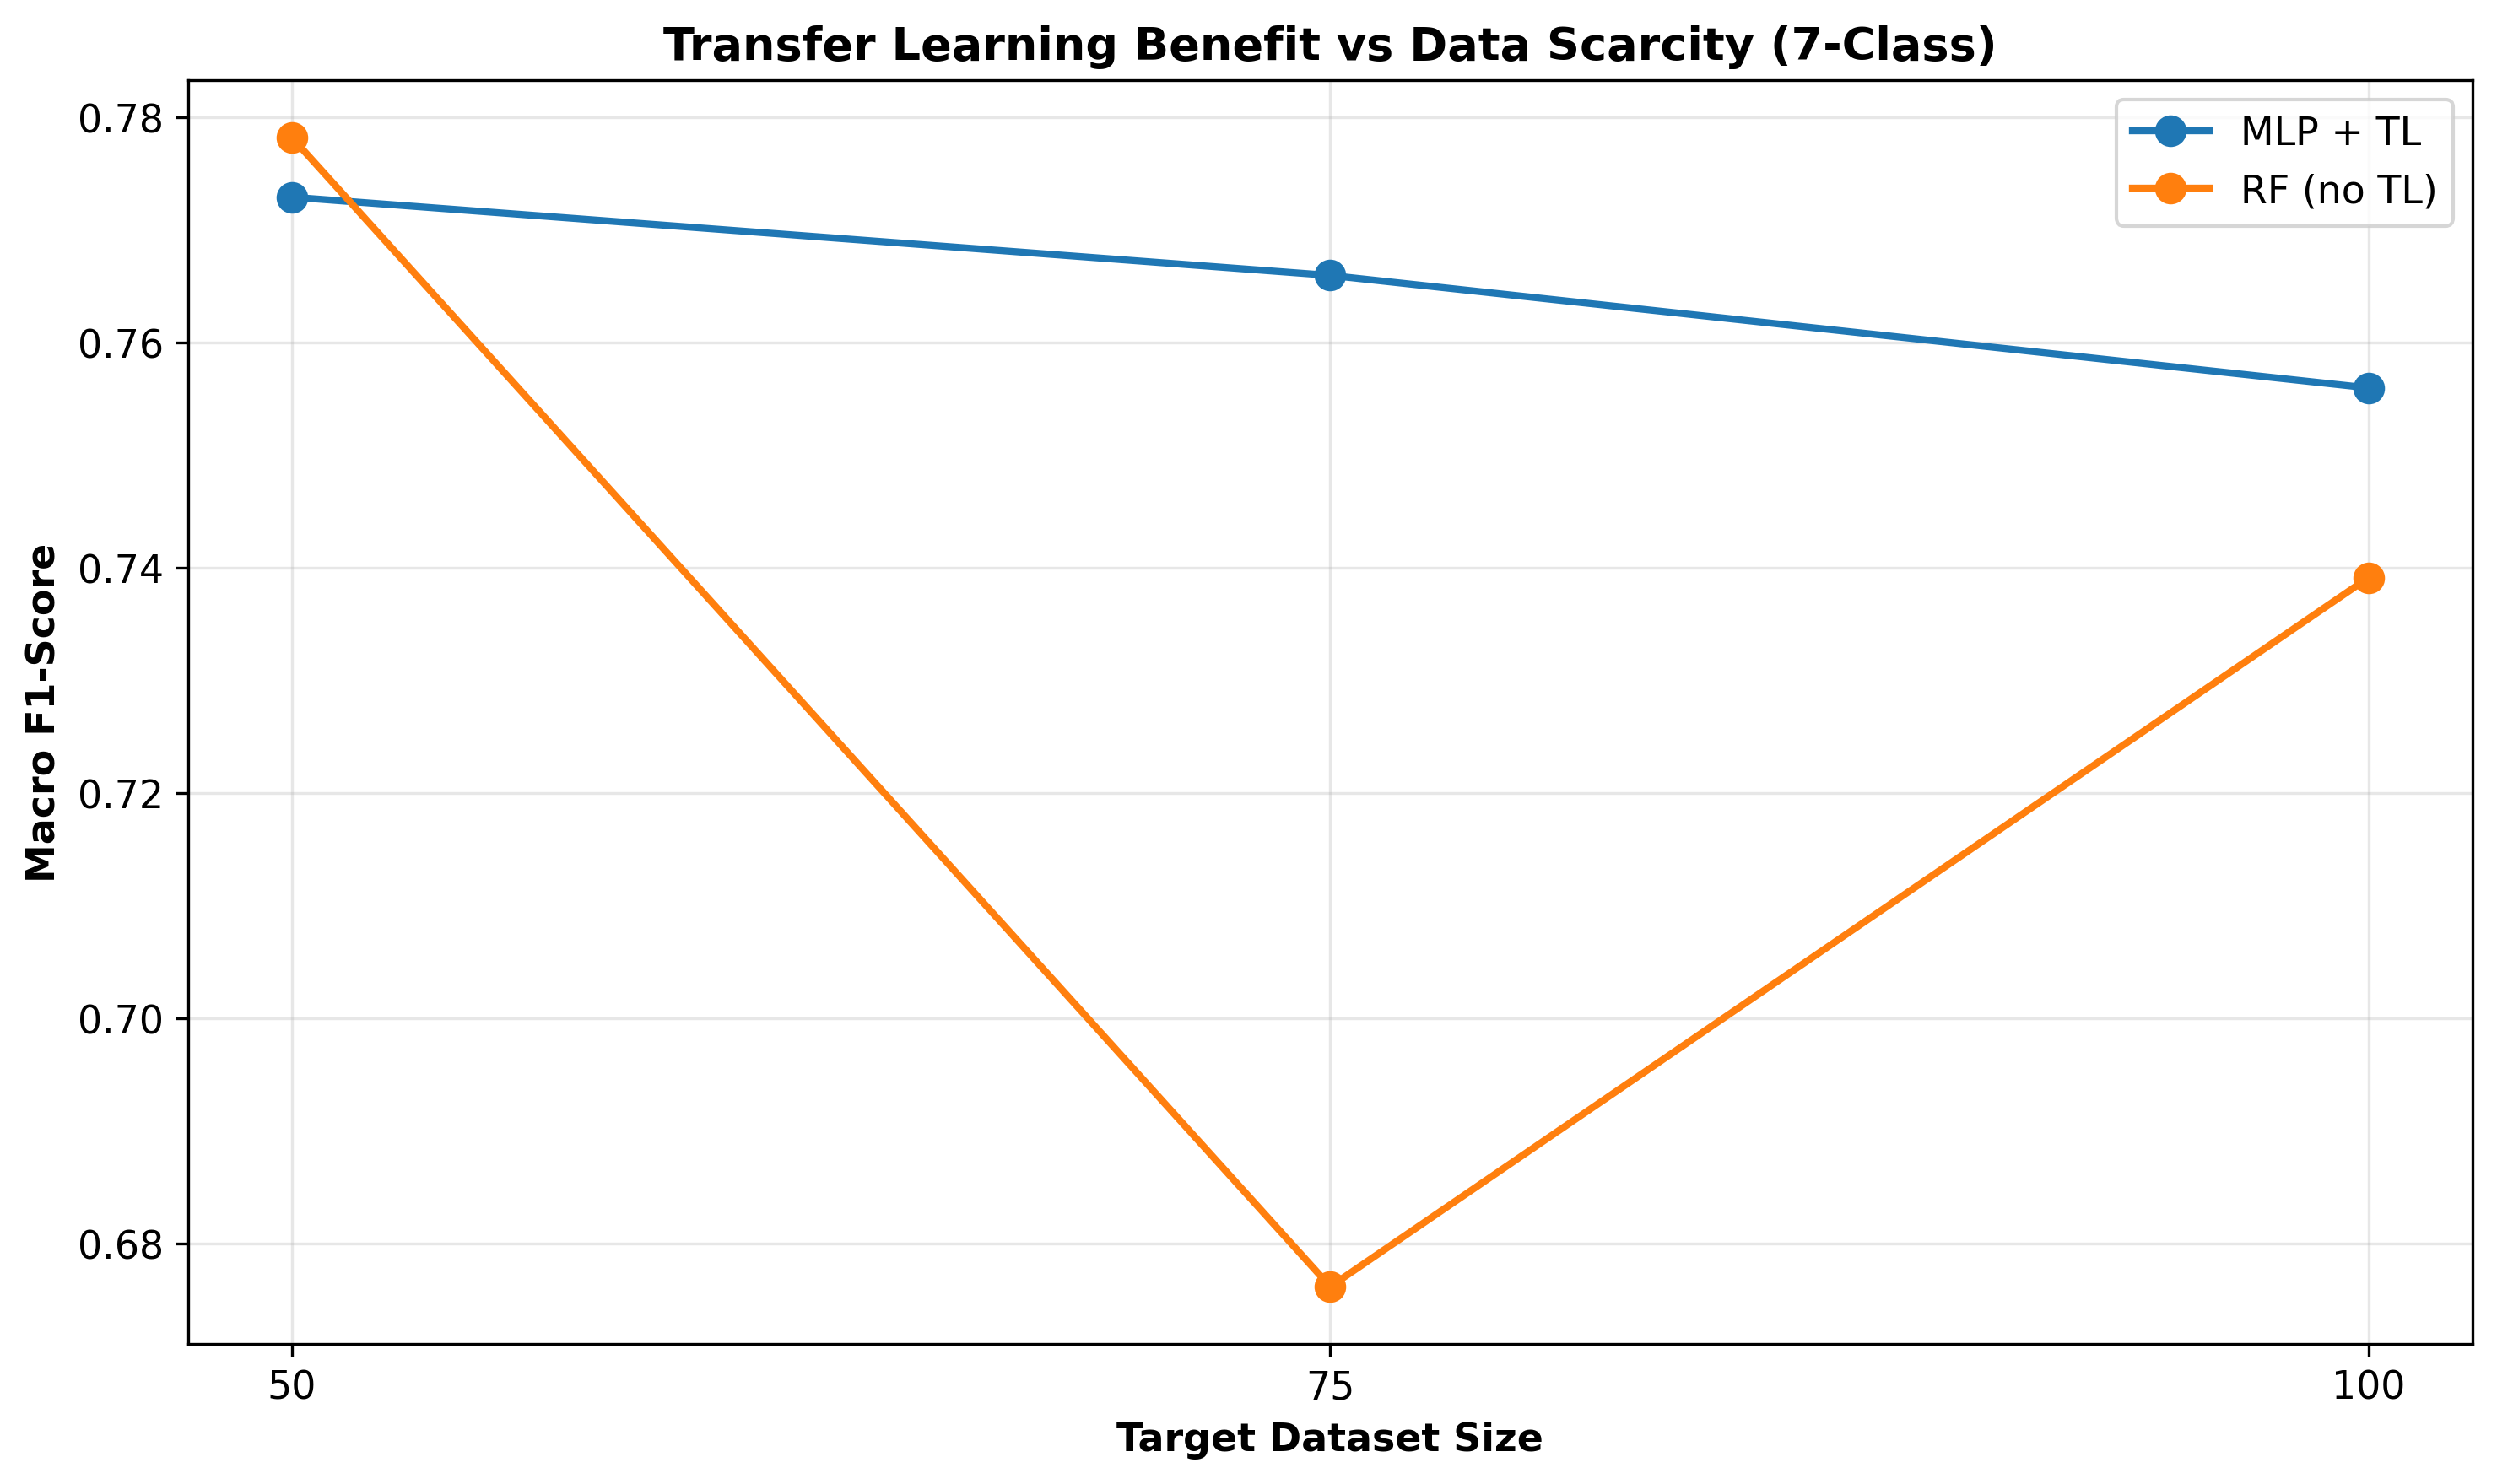
\includegraphics[width=0.95\columnwidth]{results/figures/data_scarcity_ablation.png}
  \caption{Macro-F1 vs.\ target dataset size.
           Transfer learning (MLP+TL) dominates Random Forest
           when $n_T \leq 100$ samples are available.}
  \label{fig:scarcity}
\end{figure}

\subsection{4-Class Results and Confusion Matrix Analysis}
Table~\ref{tab:results4} presents results under the simplified
four-class scheme (Discharge\,=\,D1+D2; Thermal\,=\,T1+T2+T3),
which reduces label ambiguity among closely related fault types.
RF again leads with F1\,=\,0.883, while MLP+TL (Freeze Head /
Progressive) achieves 0.769.
All methods improve by 3--8 percentage points over the 7-class
scheme, as expected from the reduced number of decision boundaries.
The TL advantage over MLP no-TL is smaller here ($+$0.5\,pp in the
4-class case vs.\ $+$9.0\,pp in the 7-class case),
suggesting that transfer learning provides the greatest benefit
for fine-grained fault discrimination.

\begin{table}[t]
  \centering
  \caption{4-Class Results (5-fold CV on $\mathcal{D}_T$, $n_T=148$).
           Discharge\,=\,D1+D2; Thermal\,=\,T1+T2+T3.}
  \label{tab:results4}
  \setlength{\tabcolsep}{4pt}
  \begin{tabular}{llcccc}
    \toprule
    Method & Type & Acc & F1 & Prec & Rec \\
    \midrule
    \textbf{Random Forest}        & Base. & \textbf{0.960} & \textbf{0.883} & \textbf{0.889} & \textbf{0.889} \\
    XGBoost                       & Base. & 0.926 & 0.845 & 0.887 & 0.843 \\
    SVM (RBF)                     & Base. & 0.866 & 0.698 & 0.694 & 0.714 \\
    kNN ($k=5$)                   & Base. & 0.811 & 0.665 & 0.699 & 0.666 \\
    \midrule
    MLP (source only)             & TL    & 0.845 & 0.781 & 0.788 & 0.819 \\
    MLP (no TL)                   & Base. & 0.892 & 0.774 & 0.787 & 0.775 \\
    MLP + TL (Freeze / Prog.)     & TL    & 0.845 & \underline{0.769} & 0.786 & 0.818 \\
    MLP + TL (Full Fine-tune)     & TL    & 0.838 & 0.758 & 0.772 & 0.792 \\
    CNN + TL (Progressive)        & TL    & 0.804 & 0.741 & 0.751 & 0.781 \\
    CNN + TL (Full / Freeze)      & TL    & 0.797 & 0.735 & 0.745 & 0.777 \\
    CNN (source only)             & TL    & 0.784 & 0.718 & 0.730 & 0.751 \\
    \bottomrule
  \end{tabular}
  \vspace{1pt}
  \small{Underlined = best TL method. Acc, F1, Prec, Rec are macro-averaged.}
\end{table}

Fig.~\ref{fig:confusion} shows the 7-class confusion matrices for
the best baseline (RF) and the best transfer-learned model
(MLP+TL Full Fine-tune).
Both models maintain high accuracy on Normal and D2 (the two
largest classes); errors concentrate in the rare-fault classes
(PD, D1), consistent with the class-imbalance motivation.
The MLP+TL model shows better recall on T1 and T2 than RF,
suggesting that source-domain pretraining improves representations
for underrepresented thermal fault types.
Fig.~\ref{fig:confusion4} confirms this pattern in the 4-class
setting, where merging thermal sub-types eliminates most T1/T2
confusion.

\begin{figure}[t]
  \centering
  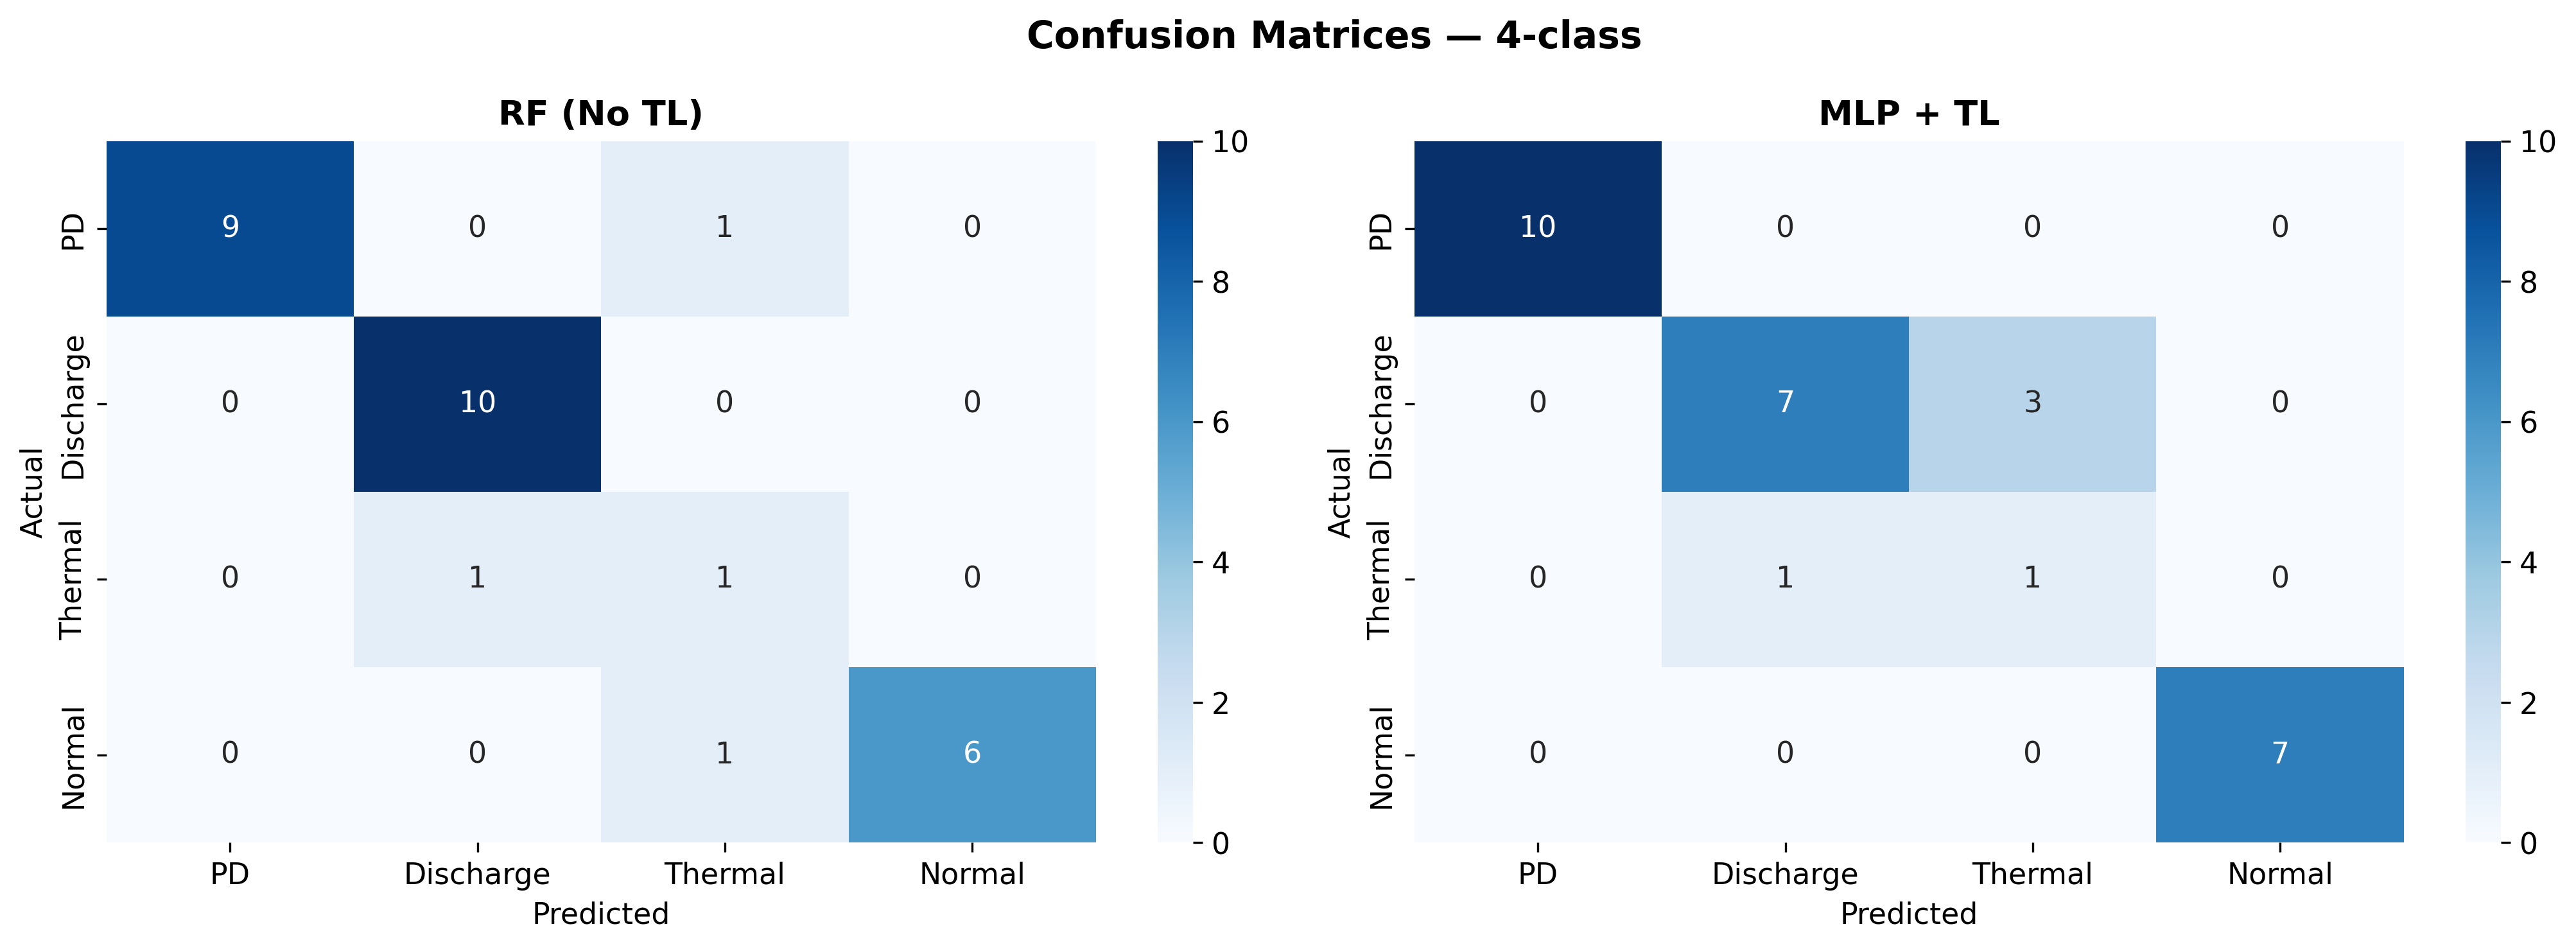
\includegraphics[width=0.98\columnwidth]{results/figures/confusion_4-class.png}
  \caption{Confusion matrices for the 4-class scheme.
           Merging thermal sub-types reduces confusion,
           yielding clearer class boundaries for both models.}
  \label{fig:confusion4}
\end{figure}

\begin{figure}[t]
  \centering
  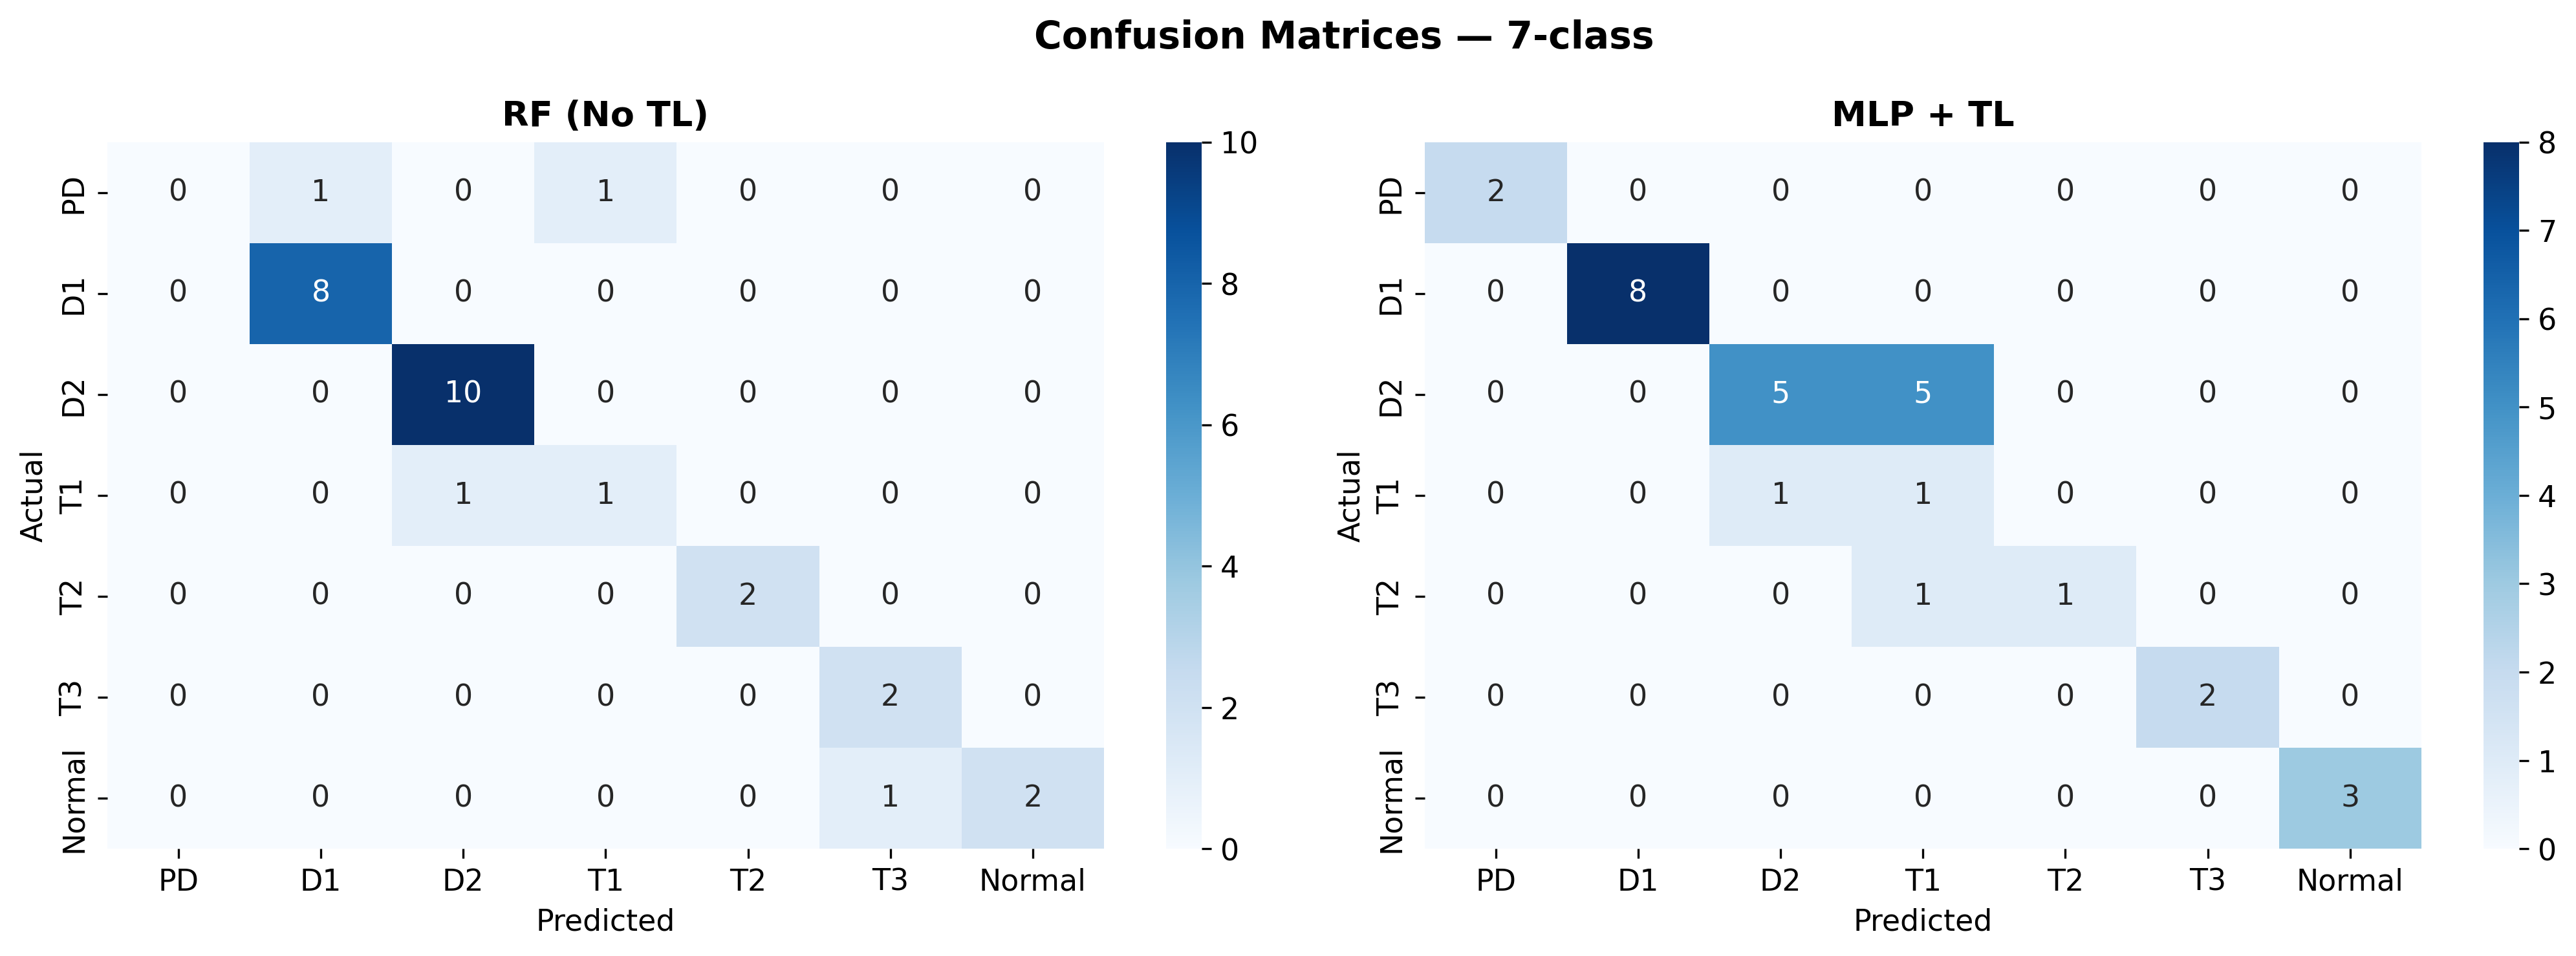
\includegraphics[width=0.98\columnwidth]{results/figures/confusion_7-class.png}
  \caption{Confusion matrices on the 7-class scheme.
           Left: Random Forest baseline (best classical model).
           Right: MLP with full fine-tune (best TL model).
           Misclassifications concentrate in rare-fault classes.}
  \label{fig:confusion}
\end{figure}

\subsection{SHAP Interpretability}
Fig.~\ref{fig:shap} compares mean $|\text{SHAP}|$ per feature for the
source-only model versus the fine-tuned model.
CO and CO$_2$ rank among the top-5 features in the adapted model,
whereas they rank below the median in the source-only model.
This shift in feature importance provides interpretable evidence that
the fine-tuning process has successfully encoded the tropical-climate
signal (elevated CO/CO$_2$) into the model representations,
corroborating the KS-test quantification of domain shift.

\begin{figure}[t]
  \centering
  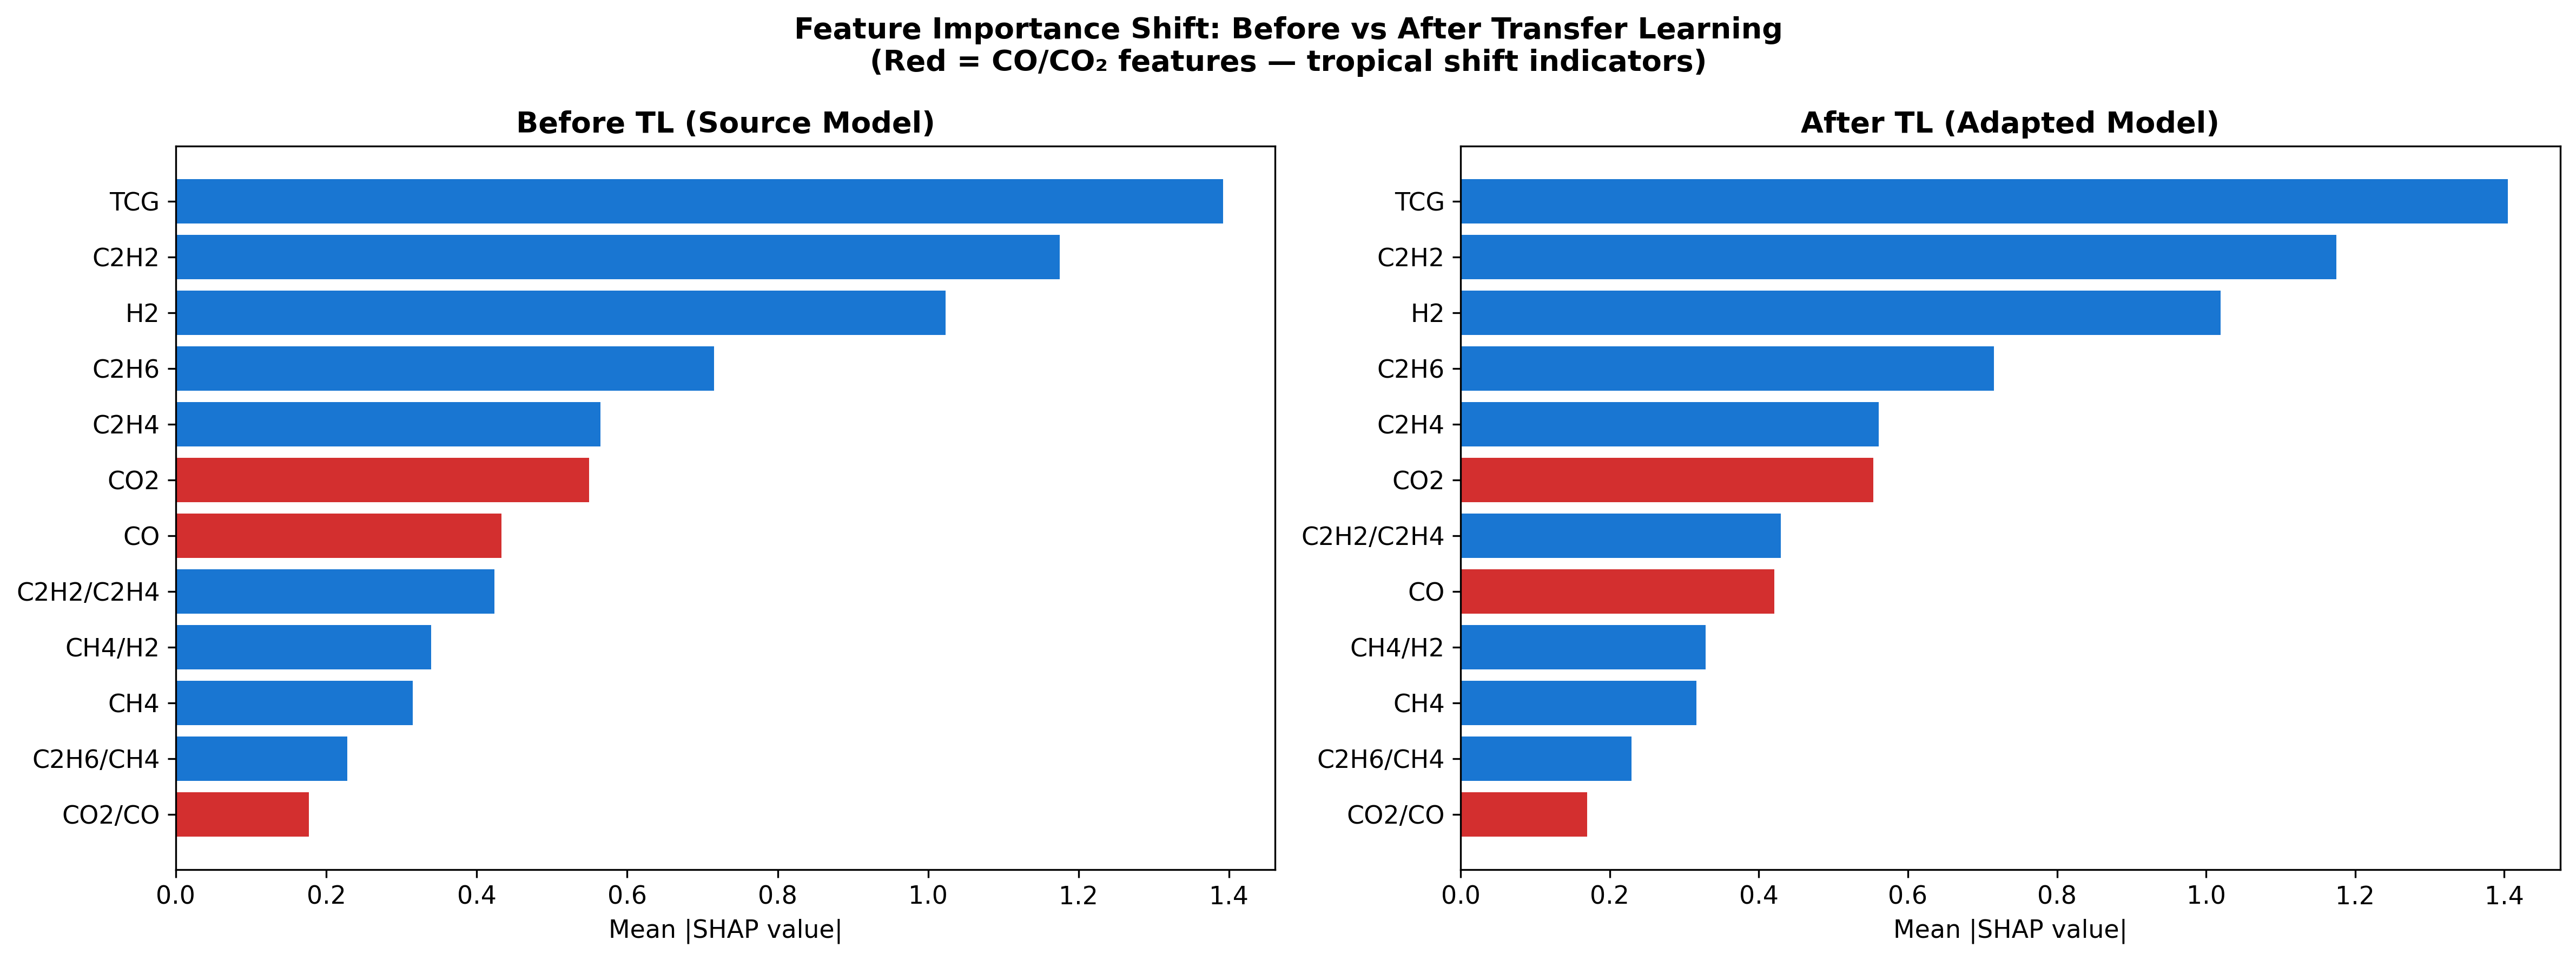
\includegraphics[width=0.95\columnwidth]{results/figures/shap_comparison.png}
  \caption{SHAP feature importance before (left) and after (right)
           transfer learning.
           CO and CO$_2$ (red bars) gain importance after
           fine-tuning on tropical target data.}
  \label{fig:shap}
\end{figure}

\subsection{Discussion of Limitations}
\label{sec:limits}
Several limitations apply to the current study.
First, all results are from a simulation using synthetic data:
gas concentrations are sampled from log-normal distributions
calibrated to IEC\,60599 ranges, and the tropical shift multipliers
for CO and CO$_2$ are approximate parameters (not directly
measured from PLN field records).
Validation on actual PLN DGA measurements is the essential next step.
Second, as noted in Section~\ref{sec:method}, the Duval Pentagon
boundaries and the CO/CO$_2$ tropical shift multipliers used in
the simulation are unverified approximations; both must be
confirmed against primary sources before the methodology is applied
to real PLN diagnosis.
Third, only macro-averaged metrics are reported; per-class F1 for
rare faults (PD, D1) is provided in the confusion matrices
(Fig.~\ref{fig:confusion}) but should be analysed in dedicated
follow-up work, since these classes are where transfer learning
is most expected to help.
Fourth, Random Forest outperforms TL methods when $n_T = 148$ samples
are available, and the difference is not statistically significant;
the TL advantage emerges only in the scarce-data regime.

% ─────────────────────────────────────────────────────────────────
\section{Conclusion}
\label{sec:conclusion}

This paper presented the first simulation-based study framing
tropical-climate CO/CO$_2$ elevation in DGA as a domain shift
problem, and proposed a transfer learning pipeline that adapts
a model pretrained on IEC TC\,10 to a small PLN Indonesia target
dataset.
Key findings from simulation experiments are:
(i)~only CO and CO$_2$ are significantly shifted (KS-test, $p < 10^{-7}$);
(ii)~transfer learning raises macro-F1 from 0.670 to 0.760 over the
no-TL MLP baseline;
(iii)~at $n_T = 75$ target samples, TL achieves a 9.0~pp F1 advantage
over Random Forest; and
(iv)~SHAP analysis confirms that CO/CO$_2$ features gain importance
after domain adaptation.

From a practical perspective, the MLP+TL model has approximately
3{,}000 parameters and runs in under one millisecond per sample on
CPU, making it deployable on PLN substation monitoring hardware
without GPU infrastructure.
The pre-model ANOVA feature ranking provides utility engineers with
an interpretable, standard-aligned view of which gas features
most discriminate fault types, complementing the post-hoc SHAP
explanations.
The auto-labeling pipeline (majority vote across six DGA
interpretation methods) enables PLN to leverage existing unlabeled
gas records for model training without requiring expert re-labeling.

Future work should (a)~validate these findings on actual PLN
field DGA records with expert-confirmed fault labels, replacing the
simulation's synthetic CO/CO$_2$ multipliers with measured values;
(b)~investigate domain-adversarial and MMD-based adaptation to
further close the source--target gap;
(c)~extend the approach to ester-insulating-oil transformers,
which exhibit different gas profiles; and
(d)~incorporate temporal DGA trends (rate of gas change) as
additional features, as recent literature suggests these carry
fault-progression information not captured by single-sample
concentrations.

% ─────────────────────────────────────────────────────────────────
\section*{Acknowledgment}
% TODO: add funding/acknowledgment here

% ─────────────────────────────────────────────────────────────────
\begin{thebibliography}{20}

% --- Verified in this study (full text or full passages read) ---
\bibitem{DladlaThango2025}
V.\,M.\,N. Dladla and B.\,A. Thango,
``Fault Classification in Power Transformers via Dissolved Gas Analysis
and Machine Learning Algorithms: A Systematic Literature Review,''
\textit{Applied Sciences}, vol.\,15, no.\,5, p.\,2395, Feb.\ 2025,
doi: 10.3390/app15052395.

\bibitem{RahmandaSuwarno2022}
D. Rahmanda and Suwarno,
``Comparison of Dissolved Gas Analysis Interpretation Methods for
Power Transformers,''
\textit{Proc.\ 3rd ITB Graduate School Conf.}, Dec.\ 2022,
pp.\,132--143, ISSN: 2963-718X.

\bibitem{SutiknoPrasojo2024}
H. Sutikno, R.\,A. Prasojo, and A. Abu-Siada,
``Machine learning based multi-method interpretation to enhance
dissolved gas analysis for power transformer fault diagnosis,''
\textit{Heliyon}, vol.\,10, 2024.
% PMC10877302 — verify DOI before submission

% --- Standards ---
\bibitem{IEC60599}
IEC, \textit{Mineral Oil-Impregnated Electrical Equipment in
Service---Guide to the Interpretation of Dissolved and Free Gases
Analysis}, IEC~60599:2022.

\bibitem{IEEEC57104}
IEEE, \textit{IEEE Guide for the Interpretation of Gases Generated
in Mineral Oil-Immersed Transformers}, IEEE Std C57.104-2019.

% --- Original method papers (well-established) ---
\bibitem{Duval2002}
M. Duval,
``A review of faults detectable by gas-in-oil analysis in transformers,''
\textit{IEEE Electr.\ Insul.\ Mag.}, vol.\,18, no.\,3, pp.\,8--17,
May 2002.
% TODO: verify DOI before submission

\bibitem{Rogers1978}
R.\,R. Rogers,
``IEEE and IEC codes to interpret incipient faults in transformers,
using gas in oil analysis,''
\textit{IEEE Trans.\ Electr.\ Insul.}, vol.\,EI-13, no.\,5,
pp.\,349--354, Oct.\ 1978.

\bibitem{Dornenburg1974}
E. Dornenburg and W. Strittmatter,
``Monitoring oil-cooled transformers by gas-in-oil analysis,''
\textit{Brown Boveri Rev.}, vol.\,61, pp.\,238--247, 1974.

% --- Imbalance handling ---
\bibitem{Chawla2002SMOTE}
N.\,V. Chawla, K.\,W. Bowyer, L.\,O. Hall, and W.\,P. Kegelmeyer,
``SMOTE: Synthetic Minority Over-sampling Technique,''
\textit{J. Artif.\ Intell.\ Res.}, vol.\,16, pp.\,321--357, 2002.
% TODO: verify DOI before submission

\bibitem{Batista2004SMOTEENN}
G.\,E.\,A.\,P.\,A. Batista, R.\,C. Prati, and M.\,C. Monard,
``A study of the behavior of several methods for balancing machine
learning training data,''
\textit{ACM SIGKDD Explor.\ Newsl.}, vol.\,6, no.\,1, pp.\,20--29,
Jun.\ 2004.

\bibitem{Wang2024SMOTE}
L.-Z. Wang \textit{et al.},
``Transformer fault diagnosis method based on SMOTE and NGO-GBDT,''
\textit{Sci.\ Rep.}, vol.\,14, p.\,7609, 2024,
doi: 10.1038/s41598-024-57509-w.

% --- Transfer learning and interpretability ---
\bibitem{PanYang2010}
S.\,J. Pan and Q. Yang,
``A survey on transfer learning,''
\textit{IEEE Trans.\ Knowl.\ Data Eng.}, vol.\,22, no.\,10,
pp.\,1345--1359, Oct.\ 2010.
% TODO: verify DOI before submission

\bibitem{LundbergLee2017SHAP}
S.\,M. Lundberg and S.-I. Lee,
``A Unified Approach to Interpreting Model Predictions,''
in \textit{Proc.\ NeurIPS}, 2017, pp.\,4765--4774.

% --- DGA + ML baselines (sourced via Dladla \& Thango 2025 SLR Table 6) ---
\bibitem{Ghoneim2016ANN}
S.\,S.\,M. Ghoneim, I.\,B.\,M. Taha, and N.\,I. Elkalashy,
``Integrated ANN-based proactive fault diagnostic scheme for power
transformers using dissolved gas analysis,''
\textit{IEEE Trans.\ Dielectr.\ Electr.\ Insul.}, vol.\,23, no.\,3,
pp.\,1838--1845, 2016.

\bibitem{Aizpurua2018Bayes}
J.\,I. Aizpurua \textit{et al.},
``Power transformer dissolved gas analysis through Bayesian networks
and hypothesis testing,''
\textit{IEEE Trans.\ Dielectr.\ Electr.\ Insul.}, vol.\,25, no.\,2,
pp.\,494--506, 2018.

\bibitem{Taha2021CNN}
I.\,B.\,M. Taha, S. Ibrahim, and D.-E.\,A. Mansour,
``Power transformer fault diagnosis based on DGA using a
convolutional neural network with noise in measurements,''
\textit{IEEE Access}, vol.\,9, pp.\,111162--111170, 2021.

\bibitem{Hoballah2020GWO}
A. Hoballah, D.-E.\,A. Mansour, and I.\,B.\,M. Taha,
``Hybrid grey wolf optimizer for transformer fault diagnosis using
dissolved gases considering uncertainty in measurements,''
\textit{IEEE Access}, vol.\,8, pp.\,139176--139187, 2020.

\bibitem{Prasojo2023RFSMOTE}
R.\,A. Prasojo \textit{et al.},
``Precise transformer fault diagnosis via random forest model
enhanced by synthetic minority over-sampling technique,''
\textit{Electr.\ Power Syst.\ Res.}, vol.\,220, p.\,109361, 2023.
% TODO: verify DOI before submission

\bibitem{Khan2015ANFIS}
S.\,A. Khan, M.\,D. Equbal, and T. Islam,
``A comprehensive comparative study of DGA based transformer fault
diagnosis using fuzzy logic and ANFIS models,''
\textit{IEEE Trans.\ Dielectr.\ Electr.\ Insul.}, vol.\,22, no.\,1,
pp.\,590--596, 2015.

% TODO: add Prasojo, Gumilang \& Suwarno (Energies 2020) once full
% paper is obtained, to support Duval Pentagon boundary verification.

\end{thebibliography}

\end{document}
